\section{ Comparison of models}\label{model_comparisons}

As mentioned in Section \ref{cnn_ref}, we used Keras Tuner model to find hyperparameters that would yield the highest accuracy.
Instead of hard-coding hyperparameters when building a model with Keras API, we defined a search space of possible values with \verb|HyperParameter| class and used that as a hyperparameter.

We passed the created model to a \verb|RandomSearch| class, with few other parameters such as batch size, number of epochs and maximum number of trials.
As we started the hyperparameter search, Keras Tuner started picking a randomly set of hyperparameters, which were used to train a model.
This process was repeated for a trial number of times.
Used hyperparameters and achieved accuracy on the validation set for each trained model were logged in a text file for later use.

After training several different models we picked a few and compared them.
Comparison of models trained in Edge Impulse Studio was also done.


\subsection{ Hyperparameter search space and results analysis}

General structure of CNN model was already described in Section \ref{cnn_ref} and in Figure \ref{model_code}.
We decided to search for the following hyperparameters: 

\begin{itemize}
    \item Number of filters in all three convolutional layers (can be different for each layer)
    \item Size of filters in all three convolutional layers (same for all layers)
    \item Size of the dense layer
    \item Dropout rate 
    \item Learning rate
\end{itemize}

Possible values of hyperparameters (also known as hyperparameter search space) are specified in Table \ref{hyper_table1}.
\newline
\begin{table}[ht]
    \centering
    \caption{ First hyperparameter search space}
    \rowcolors{2}{white}{gray!25}
    \begin{tabular}{@{} *5l @{}}    \toprule
        \textbf{Hyperparameter} & \textbf{Set of values}\\\midrule
        \verb|FilterNum1|       & From 16 to 80, with a step of 8\\ 
        \verb|FilterNum2|       & From 16 to 80, with a step of 8\\ 
        \verb|FilterNum3|       & From 16 to 80, with a step of 8\\
        \verb|FilterSize|       & 3 x 3 or 3 x 4\\
        \verb|DenseSize|        & From 16 to 96, with a step of 8\\
        \verb|DropoutRate|      & From 0.2 to 0.5, with a step of 0.05\\
        \verb|LearningRate|     & 0.0001 or 0.0003\\\toprule
        \textbf{Random search}  & \textbf{value}\\
        \textbf{variable}       & \\\midrule
        \verb|EPOCHS|           & 25\\
        \verb|BATCH_SIZE|       & 100\\
        \verb|MAX_TRIALS|       & 300\\\bottomrule
    \end{tabular}
    \label{hyper_table1}
\end{table}

Search space of \verb|FilterNumX|, \verb|DenseSize| and \verb|DropoutRate| hyperparameters were chosen based on initial training tests conducted on a thermal image dataset and other various models that were trained on similar data.
Value of \verb|FilterSize| is usually 3 x 3, however, most of example ML projects that we could find on the Internet were training on image data of the same dimensions.
We wanted to test how would a filter with the same ratio of dimensions as image data (3 x 4 and 60 x 80 respectively) perform.
Hyperparameter \verb|learning_rate| was chosen heuristically, we saw that 10 times higher values, such as 0.001 or 0.003, would leave model's accuracy stuck at suboptimal optima, from where it could not be improved anymore.

We also had to set 3 variables that directly affected how long will random search last.
From initial tests we saw that models usually reached maximum possible accuracy around \nth{20} epoch, to give some headroom we set the number of epochs to 25.
We kept batch size relatively small, at 100, which meant that weights would get updated regularly.
Hyperparameter \verb|MAX_TRIALS| had the biggest impact on the training time, we set it to 300.

The training lasted for about 12 hours. 
After it was done we compiled a list of all 300 trained models and their different hyperparameter values, number of parameters and achieved accuracies
Part of it can be seen in Table \ref{hyper_results1}.
\newline
\begin{table}[ht]
    \centering
    \caption{ Partial results of first random search of hyperparameters}
    \rowcolors{2}{gray!25}{white}
    \begin{tabular}{llllllllrl}
    \textbf{Model ID} & \rot{FilterNum1} & \rot{FilterNum2} & \rot{FilterNum3} & \rot{DenseSize} & \rot{DropoutRate}  &\rot{FilterSize} & \rot{LearningRate} & \rotatebox{45}{\parbox{2cm}{Number of parameters}} & \rot{Accuracy[\%]}  \\\toprule
        0a & 72 & 80 & 64 & 72 & 0.4  & 3x4 & 0.0003 & 1,514,400 & 98.35\\
        1a & 32 & 40 & 72 & 56 & 0.35 & 3x4 & 0.0001 & 1,260,332 & 98.31\\
        2a & 40 & 48 & 32 & 64 & 0.35 & 3x4 & 0.0001 &   656,797 & 98.31\\
        3a & 56 & 16 & 48 & 72 & 0.4  & 3x4 & 0.0001 & 1,057,924 & 98.28\\
        4a & 80 & 64 & 40 & 96 & 0.45 & 3x4 & 0.0003 & 1,245,788 & 98.28\\\midrule
       96a & 16 & 32 & 72 & 80 & 0.25 & 3x4 & 0.0001 & 1,762,508 & 98.00\\
       97a & 72 & 56 & 40 & 56 & 0.45 & 3x4 & 0.0003 &   748,580 & 98.00\\
       98a & 32 & 24 & 24 & 48 & 0.35 & 3x3 & 0.0001 &   358,308 & 98.00\\
       99a & 48 & 16 & 40 & 40 & 0.45 & 3x3 & 0.0003 &   493,412 & 98.00\\
      100a & 24 & 72 & 64 & 40 & 0.45 & 3x3 & 0.0003 &   844,684 & 98.00\\\midrule
      191a & 64 & 56 & 16 & 52 & 0.4  & 3x3 & 0.0001 &   386,996 & 97.76\\
      192a & 48 & 40 & 24 & 24 & 0.4  & 3x4 & 0.0001 &   208,172 & 97.73\\
      193a & 56 & 64 & 72 & 24 & 0.25 & 3x4 & 0.0003 &   617,692 & 97.73\\
      194a & 48 & 72 & 48 & 32 & 0.25 & 3x4 & 0.0003 &   544,652 & 97.73\\\midrule
      295a & 48 & 32 & 64 & 16 & 0.5  & 3x4 & 0.0001 &   351,012 & 95.87\\
      296a & 40 & 24 & 56 & 24 & 0.5  & 3x4 & 0.0001 &   431,572 & 95.77\\
      297a & 56 & 16 & 80 & 16 & 0.2  & 3x4 & 0.0001 &   411,020 & 95.63\\
      298a & 24 & 16 & 48 & 24 & 0.5  & 3x4 & 0.0001 &   359,924 & 94.46\\
      299a & 40 & 48 & 56 & 16 & 0.35 & 3x3 & 0.0003 &   310,860 & 82.86\\\bottomrule
    \end{tabular}
    \label{hyper_results1}
\end{table}

After analyzing results we came to several conclusions:

\begin{enumerate}
    \item We saw that almost all trained models, except for the last one, achieved accuracy above 90 \%. This proved that the general architecture of the model was appropriate for the problem.
    \item We could not see any visible correlation between a specific choice of a certain hyperparameter and accuracy. This showed that selection of hyperparameters is a non-heuristic task, at least for our particular problem.
    \item Filter of size 3 x 4 did not perform significantly better compared to one with size 3 x 3. 
    \item There is a weak correlation between the number of parameters (model's complexity) and accuracy, however, models with small size and great accuracy exist, model \textit{2a} is an example of that.
    \item First 200 models cover an accuracy range of 0.62 \%. However inside of this range model number of parameters varies hugely, for example, model \textit{192a} has more than 8 times fewer parameters than model \textit{96a}, although the difference in accuracy (0.27 \%) is negligible.
\end{enumerate}

It is apparent from results that large models are not necessary to achieve high accuracy on our training data, so we decided to run the random search of hyperparameters again.

This time we lowered the maximum and the minimum numbers of filters and size of the dense layer.
We decreased all steps from 8 to 2, thus increasing the number of possible configurations.
We decided to lower the bottom boundary of \verb|DropoutRate| from 0.2 to 0.0, which means that some models will not be using dropout layer at all.
We expected that training without dropout layer would produce suboptimal results, however, we wanted to test it.
Redefined search space for second random search can be seen in Table \ref{hyper_table2}
We increased the number of \verb|MAX_TRIALS| from 300 to 500, as we were expecting that more models will end up underfitting and also because there would be more possible options because of smaller step size.
Partial table of results of random hyperparameter search can be seen in Table \ref{hyper_results2}.

\begin{table}[ht]
    \centering
    \caption{ Second hyperparameter search space}
    \rowcolors{2}{white}{gray!25}
    \begin{tabular}{@{} *5l @{}}    \toprule
        \textbf{Hyperparameter} & \textbf{Set of values}\\\midrule
        \verb|FilterNum1|       & From 4 to 48, with a step of 2\\ 
        \verb|FilterNum2|       & From 4 to 48, with a step of 2\\ 
        \verb|FilterNum3|       & From 4 to 48, with a step of 2\\
        \verb|FilterSize|       & 3 x 3 or 3 x 4\\
        \verb|DenseSize|        & From 4 to 48, with a step of 2\\
        \verb|DropoutRate|      & From 0.0 to 0.5, with a step of 0.05\\
        \verb|LearningRate|     & 0.0001 or 0.0003\\\toprule
        \textbf{Random search}  & \textbf{value}\\
        \textbf{variable}       & \\\midrule
        \verb|EPOCHS|           & 25\\
        \verb|BATCH_SIZE|       & 100\\
        \verb|MAX_TRIALS|       & 500\\\bottomrule
    \end{tabular}
    \label{hyper_table2}
\end{table}

\begin{table}[ht]
    \centering
    \caption{ Partial results of second random search of hyperparameters}
    \rowcolors{2}{gray!25}{white}
    \begin{tabular}{llllllllrl}
    \textbf{Model ID} & \rot{FilterNum1} & \rot{FilterNum2} & \rot{FilterNum3} & \rot{DenseSize} & \rot{DropoutRate}  &\rot{FilterSize} & \rot{LearningRate} & \rotatebox{45}{\parbox{2cm}{Number of parameters}} & \rot{Accuracy[\%]}  \\\toprule
        0b & 40 & 20 & 20 & 48 & 0.25 & 3x4 & 0.0001 & 304,216 & 98.14\\
        1b & 44 & 10 & 28 & 42 & 0.2  & 3x4 & 0.0003 & 362,264 & 98.14\\
        2b & 18 & 38 & 26 & 38 & 0.1  & 3x4 & 0.0003 & 316,956 & 98.11\\\midrule
       95b & 20 & 16 & 34 & 40 & 0.3  & 3x3 & 0.0003 & 416,230 & 97.62\\
       96b & 46 & 42 & 28 & 32 & 0.4  & 3x3 & 0.0003 & 297,466 & 97.62\\
       97b & 30 & 26 & 30 & 34 & 0.2  & 3x3 & 0.0001 & 320,570 & 97.59\\\midrule
      195b & 28 & 16 & 40 & 24 & 0.1  & 3x3 & 0.0001 & 298,252 & 97.31\\
      196b & 44 & 30 & 32 & 20 & 0.3  & 3x4 & 0.0003 & 220,098 & 97.31\\
      197b & 46 & 40 & 10 & 40 & 0.1  & 3x3 & 0.0001 & 140,874 & 97.31\\\midrule
      295b & 20 &  8 & 34 & 26 & 0.3  & 3x3 & 0.0003 & 269,464 & 96.90\\
      296b & 18 & 16 & 10 & 20 & 0.3  & 3x4 & 0.0003 &  65,740 & 96.87\\
      297b &  8 & 22 & 28 & 16 & 0.1  & 3x3 & 0.0001 & 141,742 & 96.87\\\midrule
      395b & 10 & 20 & 12 & 30 & 0.0  & 3x3 & 0.0001 & 112,246 & 96.87\\
      396b & 24 & 24 & 46 & 18 & 0.2  & 3x3 & 0.0003 & 263,924 & 96.14\\
      397b &  6 & 18 & 12 & 24 & 0.4  & 3x4 & 0.0001 &  90,520 & 96.11\\\midrule
      497b & 42 & 30 & 22 &  6 & 0.4  & 3x3 & 0.0003 &  57,386 & 82.86\\
      498b &  4 &  4 & 20 & 12 & 0.4  & 3x3 & 0.0003 &  72,992 & 82.86\\
      499b & 32 & 36 & 36 &  4 & 0.15 & 3x3 & 0.0001 &  65,648 & 82.86\\\bottomrule
    \end{tabular}
    \label{hyper_results2}
\end{table}

\clearpage
Some observations:
\begin{enumerate}
    \item We can see that the accuracy of the best model \textit{0b} compared to the best model \textit{0a} from the previous search is only 0.21 \% lower, although it has about 5 times fewer parameters.
    \item Although that it might seem that \verb|FilterSize| of 3 x 4 yields best results, we did not saw a strong tendency towards 3 x 3 or 3 x 4 filter size after manually analyzing best 30 models.
    \item We can see that the worst three models have the same accuracy of 82.86 \%, same as the worst-performing model from the first random search. There are 82.86 \% images of elephants in the validation class, which means that the model probably assigned all validation images to elephant class and was satisfied with achieved accuracy.
    \item We can see that the model \textit{296b} has a quite low number of parameters, only 65,740 when compared to its neighbours.
\end{enumerate}

\subsection{ Comparison of selected, re-trained models}
    
Two random searches gave us a large number of different models to choose from.
In every other ML application where the execution time would not be a constraint, we could simply take the best performing model and be done with it.
In our case, we had to make a trade-off between model's accuracy and execution speed.

For comparison and later on device performance testing we decided to pick and retrain\footnotemark 6 models: \textit{0a}, \textit{2a}, \textit{0b}, \textit{172b}, \textit{338b} and \textit{460b}, their properties are listed in Table \ref{hyper_selection}.

Chosen models vary greatly in the number of parameters.
Models \textit{0a}, \textit{2a}, \textit{0b} have high number of parameters but their accuracy is high.
Models \textit{172b}, \textit{338b} and \textit{460b} were chosen because of their small size and reasonably good accuracy.
\footnotetext{Retraining was required as Keras Tuner module only saved hyperparameter settings during search and not each trained model.
As the weights are initially randomized, the accuracy of retrained models is going to be similar but not exact when compared to the accuracy returned by random search.}

\begin{table}[ht]
    \centering
    \caption{ Properties of selected models}
    \rowcolors{2}{gray!25}{white}
    \begin{tabular}{llllllllrl}
    \textbf{Model ID} & \rot{FilterNum1} & \rot{FilterNum2} & \rot{FilterNum3} & \rot{DenseSize} & \rot{DropoutRate}  &\rot{FilterSize} & \rot{LearningRate} & \rotatebox{45}{\parbox{2cm}{Number of parameters}} & \rot{Accuracy[\%]}  \\\toprule
        0a & 72 & 80 & 64 & 72 & 0.4  & 3x4 & 0.0003 & 1,514,400 & 98.35\\
        2a & 40 & 48 & 32 & 64 & 0.35 & 3x4 & 0.0001 &   656,797 & 98.31\\
        0b & 40 & 20 & 20 & 48 & 0.25 & 3x4 & 0.0001 &   304,216 & 98.14\\
      172b & 42 & 44 &  8 & 14 & 0.1  & 3x4 & 0.0001 &    60,672 & 97.38\\
      338b &  4 & 18 &  6 & 10 & 0.05 & 3x4 & 0.0003 &    20,290 & 96.63\\
      460b &  6 & 28 &  4 &  8 & 0.1  & 3x4 & 0.0003 &    13,114 & 93.60\\\bottomrule
    \end{tabular}
    \label{hyper_selection}
\end{table}

As we are dealing with an imbalanced dataset, where 82.86 \% of our validation data consists of elephant images, accuracy is not the best metric to use when comparing models.
Simply classifying all images into elephant class would yield an accuracy of 82.86 \%, which sounds high, although it would not actually do any classification.

When analysing the performance of a model on an imbalanced dataset it is more appropriate to use precision and recall metrics\footnotemark.
They can give us a better idea of how well the model is performing on data of specific classes.
Calculated metrics can be seen in Table \ref{precision_recall_table}, we abbreviated precision to P and recall to R for clarity.
\footnotetext{Precision tells us what percentage of data points in a specific predicted class fall into that class.
Recall tells us what percentage of data points inside a certain class were actually predicted correctly\cite{geron}.}
\begin{table}[ht]
    \caption{ Precision and recall metrics of trained models}
    \rowcolors{2}{gray!25}{white}
    \makebox[\textwidth]{%
    \begin{tabular}{lrrrrrrrrr}\toprule
        \textbf{Model ID}                 & 0a & 2a & 0b & 172b & 338b & 460b\\\toprule
        \textbf{Metrics}                &&&&&\\\toprule
        accuracy[\%]                    & \cellcolor{tbgreen} 98.18     
                                        & \cellcolor{tbgreeny}98.04   
                                        & \cellcolor{tbgreeny}98.04   
                                        & \cellcolor{tbyellow}96.80  
                                        & \cellcolor{tbyellow}96.28  
                                        & \cellcolor{tbred}   93.4 \\

        Number of parameters            & \cellcolor{tbred}  1,515K 
                                        & \cellcolor{tbyellow} 657K 
                                        & \cellcolor{tbyellow} 304K 
                                        & \cellcolor{tbyellow}  61K 
                                        & \cellcolor{tbgreeny}  20K 
                                        & \cellcolor{tbgreen}   13K\\\midrule

        P of elephant class[\%]         & \cellcolor{tbyellow}99.22     
                                        & \cellcolor{tbgreen}99.46   
                                        & \cellcolor{tbyellow}99.25   
                                        & \cellcolor{tbgreeny}99.29  
                                        & \cellcolor{tbyellow}98.80  
                                        & \cellcolor{tbred}97.80\\
        P of human class[\%]            & \cellcolor{tbgreen}96.92     
                                        & \cellcolor{tbgreeny}95.38   
                                        & \cellcolor{tbgreeny}95.38   
                                        & \cellcolor{tbyellow}92.00  
                                        & \cellcolor{tbyellow}91.69  
                                        & \cellcolor{tbred}80.31\\
        P of cow class[\%]              & \cellcolor{tbgreeny}90.99     
                                        & \cellcolor{tbgreen}93.69   
                                        & \cellcolor{tbyellow}90.09   
                                        & \cellcolor{tbyellow}84.68  
                                        & \cellcolor{tbyellow}75.68  
                                        & \cellcolor{tbred}69.37\\
        P of nature/random class[\%]    & \cellcolor{tbgreeny}77.42     
                                        & \cellcolor{tbyellow}64.52   
                                        & \cellcolor{tbgreen}79.03   
                                        & \cellcolor{tbyellow}46.77  
                                        & \cellcolor{tbyellow}59.68 
                                        & \cellcolor{tbred}40.32\\\midrule
        R of elephant class[\%]         & \cellcolor{tbgreen}99.29     
                                        & \cellcolor{tbyellow}98.80   
                                        & \cellcolor{tbgreeny}98.84   
                                        & \cellcolor{tbyellow}97.87  
                                        & \cellcolor{tbyellow}98.43  
                                        & \cellcolor{tbred}97.39\\
        R of human class[\%]            & \cellcolor{tbyellow}93.20     
                                        & \cellcolor{tbgreeny}94.51   
                                        & \cellcolor{tbgreen}95.09   
                                        & \cellcolor{tbyellow}91.44  
                                        & \cellcolor{tbyellow}89.22  
                                        & \cellcolor{tbred}85.57\\
        R of cow class[\%]              & \cellcolor{tbgreeny}94.39     
                                        & \cellcolor{tbyellow}92.04   
                                        & \cellcolor{tbgreen}96.15   
                                        & \cellcolor{tbyellow}89.52  
                                        & \cellcolor{tbyellow}84.00  
                                        & \cellcolor{tbred}81.91\\
        R of nature/random class[\%]    & \cellcolor{tbyellow}87.27     
                                        & \cellcolor{tbgreen}97.56   
                                        & \cellcolor{tbyellow}84.48   
                                        & \cellcolor{tbgreeny}93.55  
                                        & \cellcolor{tbyellow}67.27  
                                        & \cellcolor{tbred}28.09\\\bottomrule
    \end{tabular}}
    \label{precision_recall_table}
\end{table}

As we can see all six models are generally classifying elephants correctly, both precision and recall of elephant class are high, above 97 \%, which is important.
Precision and recall values of other classes are generally lower, especially for nature/random.
We can see that top three models \textit{0a}, \textit{2a} and \textit{0b} are quite similar in terms of precision and recall, which means that we can easily prefer \textit{0b}, without sacrificing accuracy. 
Models \textit{172b} and \textit{338b} perform a bit worse when compared to top three models, however, they have a low number of parameters which should translate to lower inference time.
Last model, \textit{460b}, performs the worst and it should generally not be used.

Another way to compare models performance is to look at a confusion matrix.
Figure \ref{double_cm} shows comparison between confusion matrices of \textit{0a} model on the left and \textit{460b} model on the right.
In the case of \textit{0a}, 19 elephant images were not classified correctly, and 17 images were wrongly classified as elephants.
This is not ideal, however is much better compared to performance of \textit{460b}, where 53 elephants were wrongly classified and 63 of images classified as elephants were not actually elephants.
\newline
\begin{figure}[ht]
    \begin{subfigure}{0.5\textwidth}
        \centering
        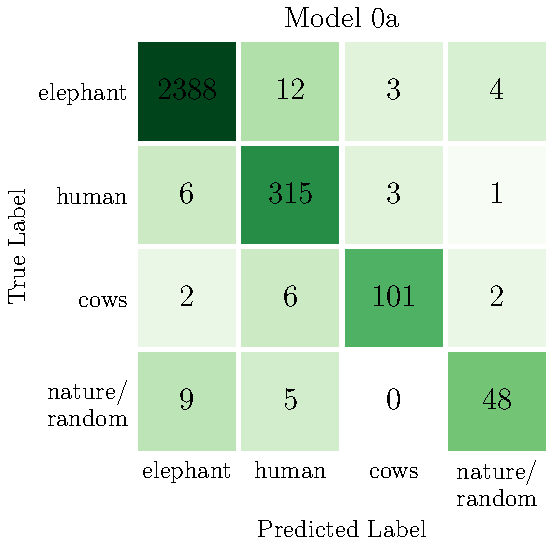
\includegraphics[width=1\linewidth]{0a_cm.pdf} 
    \end{subfigure}
    \begin{subfigure}{0.5\textwidth}
        \centering
        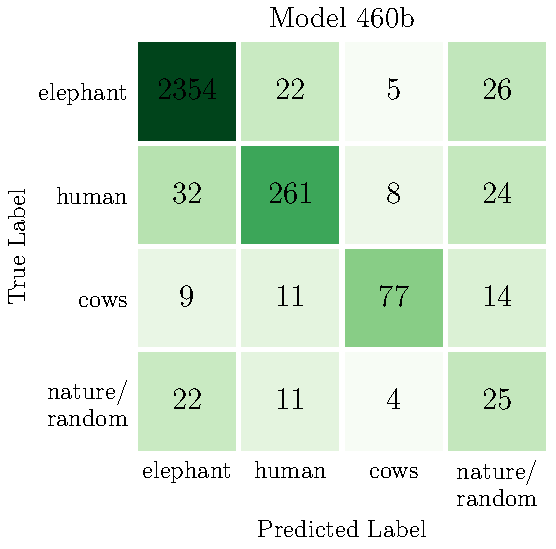
\includegraphics[width=1\linewidth]{460b_cm.pdf}
    \end{subfigure}
    \caption{Confusion matrices of \textit{0a} model (left) and \textit{460b} model (right).}
    \label{double_cm}
\end{figure}
\clearpage

\subsection{ Comparison of Edge Impulse models}

We wanted to take our 6 models and compare them against 6 Edge Impulse models that were created by using the same hyperparameters.
However, at the time of writing Edge Impulse supported only model training on images of the same dimensions.
Images with different dimensions could either be cropped or scaled to fit 1:1 ratio.
Using the same hyperparameters in Edge Impulse Studio, that were used in our models, would always create a model with a smaller number of parameters.
The smaller image creates a smaller network when compared to a bigger image, given that the rest of architecture does not change.
That meant that we could not make a direct comparison between our models and models trained in Edge Impulse Studio.
We also could not perform a random search of hyperparameters in Edge Impulse Studio, as this feature was not fully supported at the time of writing this thesis.

We decided to train a few differently sized models, using the same general CNN architecture as before, but with some minor changes in hyperparameter values.
We also trained a few models with Transfer Learning technique.
Edge Impulse offers scaled-down versions of pre-trained MobileNetV2\footnotemark NN architecture, which we used.

Tables \ref{ei_models1} and \ref{ei_models2} show properties of Edge Impulse models using CNN architecture and Transfer Learning technique, respectively. 
Table \ref{precision_recall_table_ei} shows calculated precision and recall values of Edge Impulse models using both approaches.
\footnotetext{MobileNetV2 is a efficient, lightweight NN architecture, designed for image recognition tasks, suitable for mobile applications\cite{geron}. MobileNetV2 contains width multiplier hyperparameter, which scales up or down the total number of parameters, thus providing a trade-off between accuracy and computation complexity. Edge Impulse offers three different width multiplier options: 0.35, 0.1 and 0.05.}

We used only two different versions of MobileNetV2, 0.35, and 0.1, as we saw an accuracy drop in the reduction of width multiplier hyperparameter.
In all cases the pre-trained model was followed by a one or two dense layers, with dropout layers in between.
\clearpage
\begin{table}[!htbp]
    \centering
    \caption{ Properties of Edge Impulse models using CNN architecture.}
    \rowcolors{2}{gray!25}{white}
    \makebox[\textwidth]{%
    \begin{tabular}{llllllllrl}
    \textbf{Model ID} & \rot{FilterNum1} & \rot{FilterNum2} & \rot{FilterNum3} & \rot{DenseSize} & \rot{DropoutRate}  &\rot{FilterSize} & \rot{LearningRate} & \rotatebox{45}{\parbox{2cm}{Number of parameters}} & \rot{Accuracy[\%]}  \\\toprule
        0ei & 72 & 80 & 64 & 72 & 0.4  & 3x4 & 0.0003 & 1,168,804 & 97.7\\
        1ei & 40 & 48 & 32 & 64 & 0.35 & 3x4 & 0.0001 &   503,196 & 97.5\\
        2ei & 40 & 20 & 20 & 48 & 0.25 & 3x4 & 0.0001 &   231,204 & 97.3\\
        3ei & 42 & 44 &  8 & 14 & 0.1  & 3x4 & 0.0003 &    52,272 & 96.6\\\bottomrule
    \end{tabular}}
    \label{ei_models1}
\end{table}
\bigskip
\bigskip
\bigskip
\begin{table}[!htbp]
    \centering
    \caption{ Properties of Edge Impulse models using Transfer Learning technique}
    \rowcolors{2}{gray!25}{white}
    \makebox[\textwidth]{%
    \begin{tabular}{llllllll}
        \textbf{Model ID} & \rotatebox{45}{\parbox{1cm}{Width \\Multiplier}} & \rot{DenseSize1} & \rot{DenseSize2} & \rot{DropoutRate} & \rot{LearningRate} & \rotatebox{45}{\parbox{2cm}{Number of\\parameters}} & \rot{Accuracy[\%]}  \\\toprule
        0tl & 0.35 & 16 & N/A& 0.1 & 0.0005 & 430,676 & 98.5\\
        1tl & 0.35 & 16 & 16 & 0.1 & 0.0005 & 430,948 & 98.4\\
        2tl & 0.35 & 32 & 32 & 0.1 & 0.0005 & 452,484 & 98.7\\
        3tl & 0.1  & 32 & 32 & 0.1 & 0.0005 & 135,732 & 95.7\\\bottomrule
    \end{tabular}}
    \label{ei_models2}
\end{table}
\bigskip
\bigskip
\bigskip
\begin{table}[!htbp]
    \caption{ Precision and recall metrics of trained Edge Impulse models}
    \rowcolors{2}{gray!25}{white}
    \makebox[\textwidth]{%
    \begin{tabular}{lrrrrrrrr}\toprule
        \textbf{Model ID}               & 0e    & 1e & 2e & 3e & 0tl & 1tl & 2tl & 3tl\\\toprule
        \textbf{Metrics}                &&&&&&&&\\\toprule
        Accuracy[\%]                    & \cellcolor{tbyellow} 97.7  
                                        & \cellcolor{tbyellow} 97.5  
                                        & \cellcolor{tbyellow} 97.3  
                                        & \cellcolor{tbyellow} 96.6  
                                        & \cellcolor{tbgreeny} 98.5  
                                        & \cellcolor{tbgreeny} 98.4  
                                        & \cellcolor{tbgreen} 98.7  
                                        & \cellcolor{tbred} 95.7  \\
        Number of parameters            & \cellcolor{tbred} 1,169K 
                                        & \cellcolor{tbyellow} 503K 
                                        & \cellcolor{tbgreeny} 231K 
                                        & \cellcolor{tbgreen} 52K 
                                        & \cellcolor{tbyellow} 430K 
                                        & \cellcolor{tbyellow} 431K 
                                        & \cellcolor{tbyellow} 452K 
                                        & \cellcolor{tbgreeny} 136K\\\midrule
        P of elephant class[\%]         & \cellcolor{tbgreen}  99.69 
                                        & \cellcolor{tbgreeny} 99.53 
                                        & \cellcolor{tbgreeny} 99.42 
                                        & \cellcolor{tbyellow} 99.27 
                                        & \cellcolor{tbyellow} 99.27 
                                        & \cellcolor{tbgreeny} 99.42 
                                        & \cellcolor{tbgreeny} 99.48
                                        & \cellcolor{tbred}    98.65 \\
        P of human class[\%]            & \cellcolor{tbyellow} 95.05 
                                        & \cellcolor{tbyellow} 95.05 
                                        & \cellcolor{tbyellow} 91.87 
                                        & \cellcolor{tbyellow} 91.52 
                                        & \cellcolor{tbgreen}  97.17 
                                        & \cellcolor{tbyellow} 95.41 
                                        & \cellcolor{tbgreeny} 96.47
                                        & \cellcolor{tbred}    85.16 \\
        P of cow class[\%]              & \cellcolor{tbyellow} 82.22 
                                        & \cellcolor{tbyellow} 78.89 
                                        & \cellcolor{tbyellow} 82.22 
                                        & \cellcolor{tbyellow} 79.57 
                                        & \cellcolor{tbgreen}  92.22 
                                        & \cellcolor{tbgreeny} 91.01 
                                        & \cellcolor{tbgreen}  92.22 
                                        & \cellcolor{tbred}    75.56 \\
        P of nature/random class[\%]    & \cellcolor{tbyellow} 63.04 
                                        & \cellcolor{tbyellow} 65.22 
                                        & \cellcolor{tbyellow} 73.91 
                                        & \cellcolor{tbred}    50.0  
                                        & \cellcolor{tbgreeny} 86.96 
                                        & \cellcolor{tbgreeny} 89.13 
                                        & \cellcolor{tbgreen}  91.3 
                                        & \cellcolor{tbyellow} 78.85 \\\midrule
        R of elephant class[\%]         & \cellcolor{tbgreen}  99.86 
                                        & \cellcolor{tbyellow} 98.91 
                                        & \cellcolor{tbyellow} 98.44 
                                        & \cellcolor{tbyellow} 98.65 
                                        & \cellcolor{tbgreeny} 99.48 
                                        & \cellcolor{tbgreeny} 99.27 
                                        & \cellcolor{tbgreeny} 99.37 
                                        & \cellcolor{tbred}    98.03 \\
        R of human class[\%]            & \cellcolor{tbyellow} 93.4  
                                        & \cellcolor{tbyellow} 92.44 
                                        & \cellcolor{tbgreeny} 94.2  
                                        & \cellcolor{tbred}    88.4  
                                        & \cellcolor{tbgreeny} 94.5  
                                        & \cellcolor{tbgreen}  95.74 
                                        & \cellcolor{tbgreen}  95.79 
                                        & \cellcolor{tbyellow} 90.26 \\
        R of cow class[\%]              & \cellcolor{tbyellow} 90.24 
                                        & \cellcolor{tbyellow} 86.59 
                                        & \cellcolor{tbyellow} 84.09 
                                        & \cellcolor{tbyellow} 79.57 
                                        & \cellcolor{tbgreeny} 92.22 
                                        & \cellcolor{tbyellow} 89.01 
                                        & \cellcolor{tbgreen} 94.32 
                                        & \cellcolor{tbred} 67.33 \\
        R of nature/random class[\%]    & \cellcolor{tbyellow} 87.88 
                                        & \cellcolor{tbyellow} 88.24 
                                        & \cellcolor{tbyellow} 94.44 
                                        & \cellcolor{tbgreeny} 95.83 
                                        & \cellcolor{tbgreeny} 95.24 
                                        & \cellcolor{tbgreen} 97.62 
                                        & \cellcolor{tbgreeny} 95.45 
                                        & \cellcolor{tbyellow} 91.11 \\\bottomrule
    \end{tabular}}
    \label{precision_recall_table_ei}
\end{table}
\clearpage

Some observations:
\begin{itemize}
    \item Models using CNN architecture did not out perform our models in terms of accuracy. Models \textit{2a} and \textit{0b} both had accuracy of 98.04 \%, while none of Edge Impulse models with CNN architecture did not pass 98 \%.
    \item Most of the models trained with Transfer Learning technique outperformed our models.
    \item Model \textit{2tl} performed exceptionally well, reaching an accuracy of 98.7 \% while having a relatively small number of parameters.
    \item We saw that by decreasing width multiplier we did not benefit much in accuracy as much as we lost in model size. Even increasing the sizes of dense layers did not solve the problem. 
\end{itemize}


\section{ On-device performance testing}

Performance testing of all models was done on an STM32F767ZI microcontroller, running at 216 \si{\mega\hertz}.
Testing of our models was done by using MicroML framework that we wrote, which directly called TFLite Micro API.
Testing of Edge Impulse models was done on Mbed OS, as this platform is supported by Edge Impulse and they already provide an example for it.
We could not test model \textit{0a} on device as TFLite converter failed to produce a compilable model.

To time the execution of our code we used Data Watchpoint Trigger (DWT) which contains a counter that is directly incremented by the system clock.
DWT does not use interrupts, therefore it does not introduce the overhead of calling interrupt routines as systick timer does.


Edge Impulse provides examples for testing out of the box, so not much work is needed to get the first-order approximation of performance.
For profiling, the code execution Mbed API was used, which uses timer interrupts to track elapsed time.
Figure \ref{speed_comp} shows models ranked from the fastest to the slowest.

\begin{figure}[ht]
    \centering
    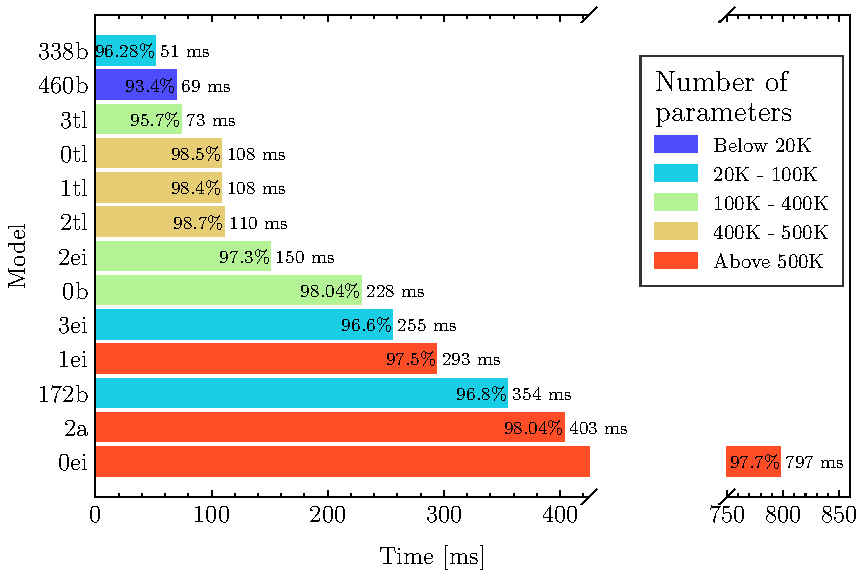
\includegraphics[width=1\linewidth]{speed_comp.pdf}
    \caption{ Comparison of time of inference of different models.}
    \label{speed_comp}
\end{figure}

We can see that all models perform inference in less than 1 second, which was a constraint that we set earlier in Section \ref{model_obj}.
Best time wise performing model was \textit{338b} with inference time of 51 \si{\milli\second}, there are also many models that perform inference under 300 \si{\milli\second}.

We also discovered some unexpected trend in results.
We assumed that inference time is proportional to the number of parameters if the general structure of the model remains the same.
As can be seen from the Figure \ref{speed_comp} there are few exceptions to this rule, model \textit{338b} executed inference faster than \textit{460b} although it has more parameters (20K versus 13K).
Model \textit{172b} was slower than \textit{0b}, although it has five times less parameters.
This behaviour is not exclusive only to our models, but it can be seen in Edge Impulse models as well, for example, models \textit{2ei} and \textit{1ei}.

Edge Impulse models trained with Transfer Learning technique \textit{0tl}, \textit{1tl}, \textit{2tl} and \textit{3tl} should not be compared to other models in this sense, as the architecture of MobileNetV2 contains additional different operations.

We can only speculate about the reason for this behaviour, since it is present both in our models and Edge Impulse models, we can assume this to be a TFLite bug.

\subsection{ Comparison of code sizes}

We also wanted to inspect Flash and RAM sizes of binaries, that we compiled for on-device testing.
For this task we used \verb|arm-none-eabi-size| command line tool which returns sizes of \verb|text|, \verb|data|, \verb|bss| sections in bytes, example of output can be seen in Figure \ref{size_output}.
To compute used Flash we need simply add bytes from \verb|text| and \verb|data| sections, and to compute used RAM we add together \verb|data| and \verb|bss| sections\footnotemark.
\lstset{style=mystyle}
\begin{figure}[ht] 
\begin{lstlisting}[language=bash]
$ arm-none-eabi-size firmware.elf
   text	   data	    bss	    dec	    hex	filename
 149124	    388	  47064	 196576	  2ffe0	firmware.elf
\end{lstlisting}
\caption{ Example output of arm-none-eabi-size command.}
\label{size_output}
\end{figure}
\footnotetext{ Data section which contains initialized static variables is first placed into Flash memory and is copied to RAM before program enters main function. That is why we have to account for additional \verb|data| section in Flash memory.}
Code sizes for all models are presented in Figure \ref{size_comp}, models are ordered the same way as they have been in Figure \ref{speed_comp}.
\begin{figure}[ht]
    \centering
    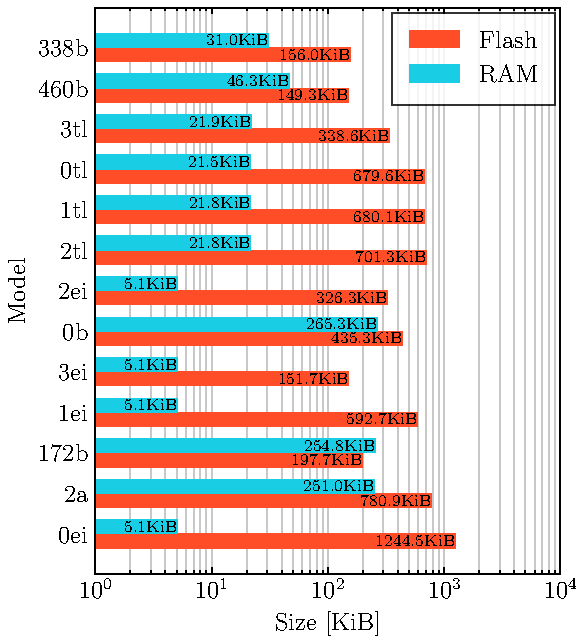
\includegraphics[width=1\linewidth]{size_comp.pdf}
    \caption{ Comparison of Flash and RAM size of compiled example models.}
    \label{size_comp}
\end{figure}

We can see that all of our models generally use more RAM then edge Impulse models.
This is due to how the inference is executed.
TFLite Micro uses a generic interpreter approach, where the model is loaded at runtime.
Edge Impulse uses a compiled approach, which they named The EON\textsuperscript{TM} Compiler\cite{eon}.
The EON\textsuperscript{TM} Compiler still uses TFLite Micro, however, it does not use its interpreter, but directly calls operation kernels.
This means that linker knows exactly which operations are used and more data can be moved into Flash, thus eliminating unneeded code space\cite{eon}.


\subsection{ Comparison of different optimisation options}

To be able to run the ML inference at maximum possible efficiency under MicroML some extra amount of work and research was required.
Figure \ref{opt_comp} shows reductions in inference time of \textit{0b} model while using different optimisation methods.
\newline

\begin{figure}[ht]
    \centering
    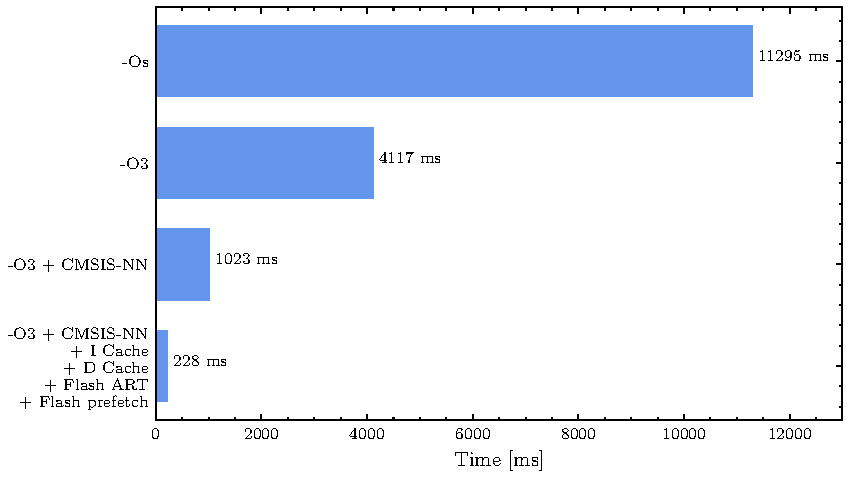
\includegraphics[width=1\linewidth]{opt_comp.pdf}
    \caption{ Inference time of \textit{0b} model using different optimisations.}
    \label{opt_comp}
\end{figure}

We started with no optimisations at all, while using only \verb|-Os| compiler flag.
\verb|-Os| flag generally optimises for minimal size, it enables all \verb|-O2| optimisations, except those that increase size.
This optimisation level is often used, however, we found out that inference time of more than 11 seconds was too long.

Changing optimisation level to \verb|-O3| drastically decreased the time of inference, down to 4117 \si{\milli\second}.
\verb|-O3| turns on all \verb|-O2| optimisations plus additional ones and completely disregards any code size optimisations.

Changing compiler optimisations flags could not lower time of inference any further, so other approaches were needed.
While reading through TensorFlow documentation we saw that it supports CMSIS-NN library for ARM microcontrollers.
CMSIS-NN is a collection of efficient Neural Network kernels, that intends to maximise performance and lower code size of NN models implemented on ARM microcontrollers.
TensorFlow provides wrappers for some of these kernels, such as convolutional, fully connected, pooling layers and others.
Not much work was needed to use these highly efficient kernels, we only needed to specify in our Makefile that we want to compile CMSIS-NN kernels and not compile generic TensorFlow kernels. 
Time of inference dropped for about 3 seconds, down to 1023 \si{\milli\second}.

As we saw that similarly sized Edge Impulse models were running much faster on Mbed platform compared to our MicroML code, while using the same microcontroller, we knew that there was another step left.
The final performance increase was reached by using features only fully found in Cortex-M7 microcontrollers and partly in Cortex M3/4 microcontrollers. 
To achieve it we had to enable I and D caches, flash prefetch and flash ART.

ART stands for Adaptive real-time memory accelerator, which encompasses I/D caches and flash prefetch buffer.
I and D caches are small, efficient portions of memory, which are located in the CPU of the microcontroller.
They hold instructions and data respectively, if those are requested by next microcontroller instruction, they can be read much faster compared to reading them from flash memory. 
By enabling flash prefetch microcontroller reads additional sequential instructions into prefetch buffer, thus enabling execution without any wait states (if instruction flow is sequential).
Elimination of wait states greatly improved the time of inference, it was decreased to 228 \si{\milli\second}.


\subsection{ Scoring trained models}\label{scoring_models}

Choosing the best model for on-field deployment is a hard task due to many different metrics: precision and recall values, time of inference, and code size.
To make this job easier we devised a scoring system: each metric is going to be normalized and multiplied with some weight value.
All products would then be summed up and the result would represent the final score.
The Sum of the weights is equal to 100, which means that the possible maximum score is also 100.
We decided to allocate 50 weight points to all precision and recall values, 30 points to the time of inference value, 5 points for Flash size and 15 points for RAM size.
As we care more about precision and recall values of elephant, human and cow classes we gave them 7 weight points each, while nature/random class received only 4.
We value Flash size less than RAM, as most of the microcontrollers have much less RAM than they do Flash, thus we gave 15 weight points to RAM size and only 5 to Flash size.

Since the time of inference, Flash and RAM sizes are properties, which should give a larger score, the smaller they are, we mapped them into a range between 0 and 1.
The smallest value inside the set would be assigned 1, the biggest 0, the values in between are mapped linearly.

Scoring is described mathematically in \ref{score_equ}, while the final results can be seen in Figure \ref{score_comp}
\begin{equation}\label{score_equ}
    \begin{aligned}
        Score[i] ={} & 7 K(P_{elephant},i) + 7 K(P_{human},i) + 7 K(P_{human},i) + 4 K(P_{ntr/rnd},i) \\
                     & +{} 7 K(R_{elephant},i) + 7 K(R_{human},i) + 7 K(R_{human},i) + 4 K(R_{ntr/rnd},i) \\
                  & +{} 30\: F(ToI, i) +5\: F(Flash, i) + 15\: F(RAM, i)   \\
                  & \\
        K(X, i) ={}  & \frac{(X[i] - MIN(X))}{MAX(X)- MIN(X)} \\
                  & \\
        F(X, i) ={}  & \frac{(X[i] - MAX(X))}{MIN(X)- MAX(X)}
    \end{aligned}
\end{equation}
\clearpage
Where:\\
$Score$ - Vector of calculated scores\\
$i$ - i$^{th}$ model\\
$P_{j}$ - Vector of precision values of j$^{th}$ class\\
$R_{j}$ - Vector of recall values of j$^{th}$ class\\
$ToI$ - Vector of Time of Inference values\\
$Flash$ - Vector of Flash sizes\\
$RAM$ - Vector of RAM sizes\\
$K(X,i)$ - Normalizing function with vector X and element index i as arguments\\
$F(X,i)$ - Normalizing, inverting, function with vector X and element index i as arguments\\
$MAX(X)$ - Function that finds maximum element in vector X\\
$MIN(X)$ - Function that finds minimum element in vector X

\begin{figure}[ht]
    \centering
    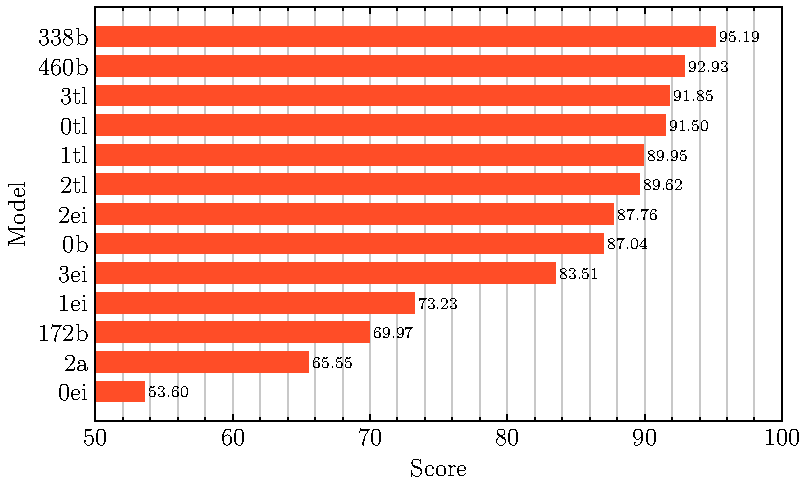
\includegraphics[width=1\linewidth]{score_comp.pdf}
    \caption{ Inference time of \textit{0b} model using different optimisations.}
    \label{score_comp}
\end{figure}

Final verdict: model \textit{3tl} received the highest score, models \textit{1tl}, \textit{2tl} follow.
This should not be a surprise, models trained with Transfer Learning achieve high accuracies and execute inference in about 100 ms or less while compiled approach for computing Neural Networks keeps used Flash and RAM sizes to a minimum.


\section{ Power profiling of an embedded early warning system}
%
%To write this section you need to:
% - wirte uart communication channel for zephyr and your system, has to be simple dont lose time on this.
% - Basic parsing of results and packing them into lora payload
% - Zephyr, put system to sleep and wake it up with pir, turn on fet.
% - Make an image with flir and do inference on it, (subtract mean image, you could test this on real dataset, without subtracted mean)
%
%- [ ] Power consumption test of whole setup, 
%      PIR wakes up wisent, 
%      wisent turns on stm32f7 and flir, 
%      which makes a picture, does inference, reports result and wisent sends the result. 
%      Otii image of consumption with marked sections.(shouldnt be hard)
%
%\subsection{ Battery life estimations}
%Based on numbers and different scenarios estimate how long would this last with different batteries.
